\newpage
\section{From Digital Electronics to Quantum Computers}

\subsection{Digital Electronics}
$A$, $B$, $\bar{A}$, $A\cdot B$, $A+B$. 

ALU. 但量子不可克隆, 所以任何分支都不太行.

\subsection{Quantum Gates}
A quantum gate is a reversible operation that a quantum computer can perform upon qubits.
 
A gate is a linear transformation on the state of the qubit that takes unit vectors into unit vectors. Such a transformations $u$ is called \textbf{unitary} and satisfies the condition
\begin{align*}
    uu^\dagger=u^\dagger u=1
\end{align*}

We begin with single-qubit gates. Note that the NOT operation X is the only nontrivial reversible operation a classical computer can perform on a single bit. 
\begin{enumerate}
    \item NOT gate (Pauli X matrix):
    \begin{align*}
        X&=\begin{pmatrix}
            0& 1 \\ 1 & 0
        \end{pmatrix}\\
        X\ket{0}&=\ket{1}\\
        X\ket{1}&=\ket{0}
    \end{align*}
    NOT gate flips the qubit, just like a classical bit.
    \item Hadamard gate can flip the qubit half way, such that we have a superposition of 0 and 1. 
    \begin{align*}
        H&=\frac{1}{\sqrt{2}}\begin{pmatrix}
            1 & 1 \\ 1 & -1
        \end{pmatrix}\sim\sqrt{NOT}\\
        H\ket{0}&=\frac{1}{\sqrt{2}}(\ket{0}+\ket{1})\\
        H\ket{1}&=\frac{1}{\sqrt{2}}(\ket{0}-\ket{1})
    \end{align*}
    Hardmard gates are often used to implement quantum parallelism. 
    \item We can also shift the phase of the qubit by a rotation around z axis. Pauli Z matrix:
    \begin{align*}
        Z&=\begin{pmatrix}
            1 & 0 \\0&-1
        \end{pmatrix}\\
        Z(a\ket{0}+b\ket{1})&=a\ket{0}-b\ket{1}
    \end{align*}
\end{enumerate}

Next, we discuss the quantum version of a controlled-NOT (CNOT) gate, which is a two-qubit gate. (可以主动提供纠缠)
\begin{itemize}
    \item If the state of the $i$th qubit (the control qubit) is $\ket{0}$, $C_{ij}$ leaves the state of the $j$th qubit (the target qubit) unchanged.
    \item If the state of the control qubit is $\ket{1}$, $C_{ij}$ applies the NOT operator X to the state of the target qubit.
\end{itemize}

e.g. 
\begin{align*}
    &C_{12}(a\ket{00}+b\ket{01}+c\ket{10}+d\ket{11})\\
    =&a\ket{00}+b\ket{01}+c\ket{11}+d\ket{10}
\end{align*}

Matrix representation:
\begin{align*}
    C_{12}=\begin{pmatrix}
        1 & 0& 0&0\\
        0 & 1& 0&0\\
        0 & 0& 0&1\\
        0 & 0& 1&0\\
    \end{pmatrix},\ C_{21}=\begin{pmatrix}
        1 & 0& 0&0\\
        0 & 0& 0&1\\
        0 & 0& 1&0\\
        0 & 1& 0&0\\
    \end{pmatrix}
\end{align*}

\subsection{Application: Quantum Teleportation}
Teleportation is not the transfer of an object by disappearing it from one point in space and reappearing it in another location. It is a transfer of the information that fully characterizes all properties of the object.

Suppose Alice has a qubit in an unknown state $\ket{\psi}_A=a\ket{0}+b\ket{1}$. In teleportation, her goal is to transfer the information (i.e. $a$ and $b$), not the physical qubit, to Bob at a different location.

(这里的分支相当于不变的演化)

\begin{figure}[H]
    \centering
    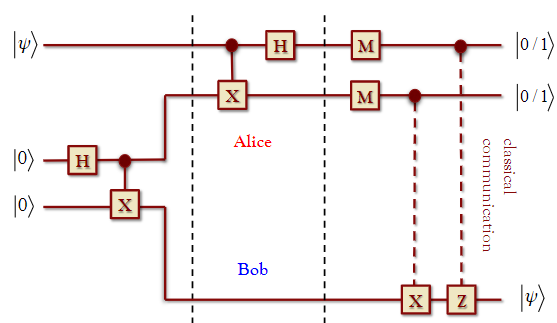
\includegraphics[width=0.479\textwidth]{QI7/Stage 1}
    \caption{Quantum Teleportation}
\end{figure}

After Stage 1:
\begin{align*}
    \ket{\Psi}&=(a\ket{0}+b\ket{1})\otimes\frac{1}{\sqrt{2}}(\ket{00}+\ket{11})\\
    &=\frac{1}{\sqrt{2}}(a\ket{000}+a\ket{011}+b\ket{100}+b\ket{111})
\end{align*}

After Stage 2:
\begin{align*}
    \ket{\Psi}=\frac{1}{2}(&a\ket{000}+a\ket{100}+a\ket{011}+a\ket{111}+\\
    &b\ket{010}-b\ket{110}+b\ket{001}-b\ket{101})\\
    \ket{\Psi}=\frac{1}{2}[&\ket{00}(a\ket{0}+b\ket{1})+\ket{01}(a\ket{1}+b\ket{0})+\\
    &\ket{10}(a\ket{0}-b\ket{1})+\ket{11}(a\ket{1}-b\ket{0})]
\end{align*}
\begin{align*}
    \ket{\Psi}=\frac{1}{2}\left[\ket{00}I+\ket{01}X+\ket{10}Z+\ket{11}XZ\right](a\ket{0}+b\ket{1})
\end{align*}

Alice has no knowledge of the quantum state, even though she is able to teleport it. 

Nor does Alice maintain a copy of the quantum state. After the teleportation, the original qubit ends up either in $\ket{0}$ or $\ket{1}$, depending on the measurement result. 

The classical communication channel is limited by the speed of light, so quantum teleportation cannot be accomplished faster than the speed of light.


\subsection{Toward a Working Quantum Computer}
\begin{itemize}
    \item\small Josephson junctions
    \item\small Trapped ions
    \item\small Photons
    \item\small Quantum dots
    \item\small NMR
    \item\small NV-centers in diamond
    \item\small Rydberg atom arrays
    \item\small Impurity spins in
    \item\small semiconductors
    \item\small Atoms and cavity QED
    \item\small Majoranas in quantum
    \item\small wires
    \item\small and more . . .
\end{itemize}

Five criteria for physical implementation of a quantum computer: 
\begin{enumerate}
    \item\small Well defined extendible qubit array-stable memory
    \item\small Preparable in the ``000...'' state
    \item\small Long decoherence time ($>10^4$ operation time)
    \item\small Universal set of gate operations
    \item\small Single-quantum measurements
\end{enumerate}

\subsubsection{Universal Quantum Gates}
A set of gates is said to be universal for quantum computation if any unitary operation may be approximated to arbitrary accuracy by a quantum circuit involving only those gate. 
\begin{enumerate}
    \item\small Any single-qubit unitary transformation can be approximated. 
    \item\small Any two-qubit unitary transformation can be approximated. 
    \item\small Any multi-qubit unitary transformation can be decomposed into a circuit of single- and two-qubit gate
\end{enumerate}

An example of a standard set is:
\begin{align*}
    \text{Hadamard gate: } H&=\frac{1}{2}\begin{pmatrix}
        1 & 1 \\ 1 & -1
    \end{pmatrix}\\
    \frac{\pi}{4}\text{ (phase) gate: } S&=\begin{pmatrix}
        1 &0\\0&i
    \end{pmatrix}\text{(not necessary)}\\
    &=e^{i\pi/4}\begin{pmatrix}
        e^{-i\pi/4} & 0 \\ 0 & e^{i\pi/4}
    \end{pmatrix}\\
    \frac{\pi}{8}\text{ gate: } S&=\begin{pmatrix}
        1 &0\\0&e^{i\pi/4}
    \end{pmatrix}\\
    &=e^{i\pi/8}\begin{pmatrix}
        e^{-i\pi/8} & 0 \\ 0 & e^{i\pi/8}
    \end{pmatrix}\\
    \text{CNOT gate: } C_{12}&=\begin{pmatrix}
        1 & 0& 0&0\\
        0 & 1& 0&0\\
        0 & 0& 0&1\\
        0 & 0& 1&0\\
    \end{pmatrix}
\end{align*}

\subsubsection{Superconducting Circuits}
A Cooper pair box qubit has a voltage source biasing the box through a coupling (`gate') capacitor. Tunable by gate and flux.

Circuit QED engineers superconducting qubits as artificial atoms coupled to microwave resonators (typically, with a single mode).

\subsubsection{Fault-Tolerant Quantum Computing}
Redundancy in coding offers possibilities to detect errors.

Microsoft is supporting a completely new quantum computing scheme, in which information is store globally in the wave function topology of an engineered system.

\subsubsection{Quantum Algorithm}
Early algorithms provided clear, but often not practical, evidences that quantum advantages exist. Quantum supremacy using a programmable superconducting processo. 

In the so-called NISQ era, hybrid classical-quantum algorithms may greatly enhance our computational capabilities (perhaps, with a probability).